% !TEX TS-program = pdflatex
% !TEX encoding = UTF-8 Unicode

% This is a simple template for a LaTeX document using the "article" class.
% See "book", "report", "letter" for other types of document.

\documentclass[12pt]{article} % use larger type; default would be 10pt

\usepackage[utf8]{inputenc} % set input encoding (not needed with XeLaTeX)

%%% Examples of Article customizations
% These packages are optional, depending whether you want the features they provide.
% See the LaTeX Companion or other references for full information.

%%% PAGE DIMENSIONS
\usepackage{geometry} % to change the page dimensions
\geometry{a4paper} % or letterpaper (US) or a5paper or....
\geometry{margin=1.1in} % for example, change the margins to 2 inches all round
% \geometry{landscape} % set up the page for landscape
%   read geometry.pdf for detailed page layout information

\usepackage{graphicx} % support the \includegraphics command and options

% \usepackage[parfill]{parskip} % Activate to begin paragraphs with an empty line rather than an indent

%%% PACKAGES
\usepackage{booktabs} % for much better looking tables
\usepackage{array} % for better arrays (eg matrices) in maths
\usepackage{paralist} % very flexible & customisable lists (eg. enumerate/itemize, etc.)
\usepackage{verbatim} % adds environment for commenting out blocks of text & for better verbatim
\usepackage{subfig} % make it possible to include more than one captioned figure/table in a single float
% These packages are all incorporated in the memoir class to one degree or another...

%%% HEADERS & FOOTERS
\usepackage{fancyhdr} % This should be set AFTER setting up the page geometry
\pagestyle{fancy} % options: empty , plain , fancy
\renewcommand{\headrulewidth}{0pt} % customise the layout...
\lhead{}\chead{}\rhead{}
\lfoot{}\cfoot{\thepage}\rfoot{}

%%% SECTION TITLE APPEARANCE
\usepackage{sectsty}
\allsectionsfont{\sffamily\mdseries\upshape} % (See the fntguide.pdf for font help)
% (This matches ConTeXt defaults)

%%% ToC (table of contents) APPEARANCE
\usepackage[nottoc,notlof,notlot]{tocbibind} % Put the bibliography in the ToC
\usepackage[titles,subfigure]{tocloft} % Alter the style of the Table of Contents
\renewcommand{\cftsecfont}{\rmfamily\mdseries\upshape}
\renewcommand{\cftsecpagefont}{\rmfamily\mdseries\upshape} % No bold!

\usepackage{cite}
\usepackage{hyperref}
\usepackage{parskip}
\usepackage{wrapfig}

\usepackage{indentfirst}
\usepackage{setspace}

\usepackage{tikz}
\usetikzlibrary{chains,fit,shapes}
\usetikzlibrary{arrows,positioning}
\usetikzlibrary{decorations.markings}

\setlength{\parindent}{1.0cm}

%%% END Article customizations

%%% The "real" document content comes below...


\author{Joshua Payne}
%\date{} % Activate to display a given date or no date (if empty),
         % otherwise the current date is printed 

\begin{document}


\begin{titlepage}

\begin{center}

\textit{\textbf{\Large MIT Department of Nuclear Engineering}} \\[3.0cm]

\large

Thesis Prospectus

For the Degree of

Master of Science 

Joshua Payne\\[1.5cm]

\textit{Implementation and Performance Evaluation of a GPU Particle-in-Cell Code}\\[2.0cm]

\normalsize
Approved by:\underline{\hspace{5.5cm}}
\\ \hspace{2.0cm} Thesis Supervisor \\[1.0cm]

Approved by:\underline{\hspace{5.5cm}}
\\ \hspace{2.0cm} Thesis Reader \\[1.0cm]

Author:\underline{\hspace{6.4cm}} \\[1.0cm]

Date:\underline{\hspace{6.9cm}} \\[1.0cm]

\end{center}
\begin{flushright}
{\today}
\end{flushright}
\end{titlepage}

\doublespacing
\section{Introduction}

Simulating plasma behavior can be incredibly difficult. The equations that govern plasma behavior are incredibly non-linear due to significance of self forces. One of the best ways to simulate plasma behavior is by simulating the behavior of individual particles. Tracking the movements and interactions of a small fraction of the $10^{20}/m^3+$ particles can provide a very accurate representation of the bulk behavior of a real plasma. This is the primary purpose of the particle in cell (PIC) method. PIC methods employ mixed particle tracking and field solving in order to solve for self consistent plasma behavior. The general PIC method is as follows;

\begin{figure}[h]
\begin{center}
%\documentclass[a4paper,5pt]{article}
%\usepackage{tikz}
%\usetikzlibrary{arrows,positioning} 


%\begin{document}

\noindent
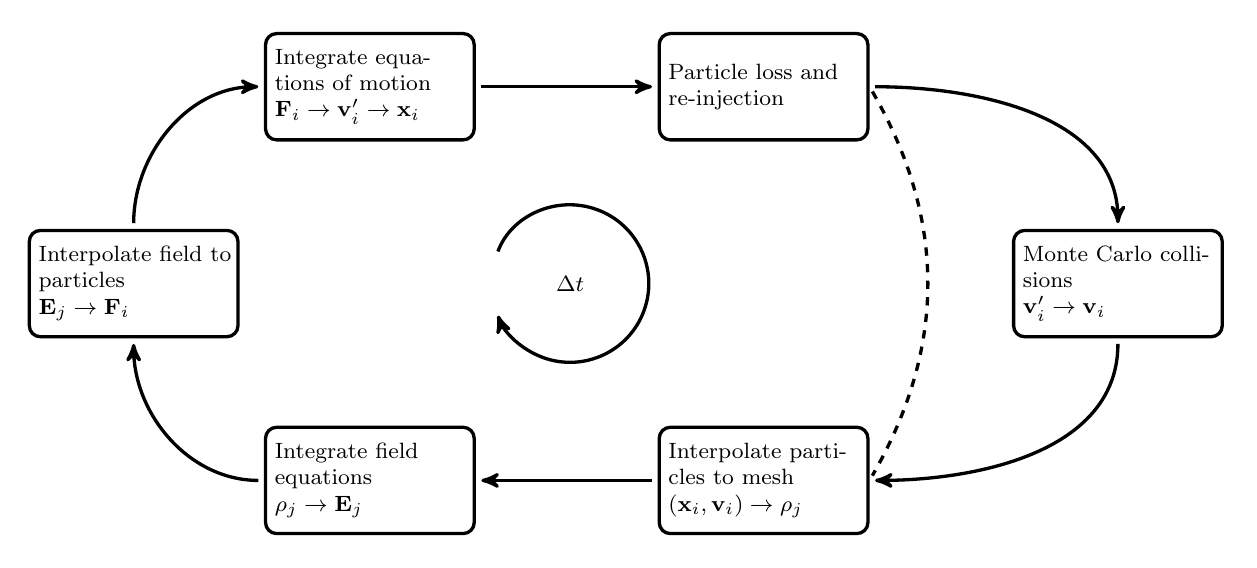
\begin{tikzpicture}[node distance=1cm,font=\footnotesize,auto]
\tikzset{
    %Define standard arrow tip
    >=stealth',
    %Define style for boxes
    punkt/.style={
           rectangle,
           rounded corners,
           draw=none, very thick,
           text width=2.5cm,
			  minimum width=2.6cm,
           minimum height=1.5cm,
			  },
    % Define arrow style
    pil/.style={
           ->,
           very thick,
           shorten <=2pt,
           shorten >=2pt,},
    punkt2/.style={
           rectangle,
           rounded corners,
           draw=black, very thick,
			  minimum width=2.65cm,
           minimum height=1.35cm,
			  anchor=west},
    punkt3/.style={
           rectangle,
           rounded corners=15pt,
           draw=black,
			  minimum width=3.2cm,
           minimum height=2.0cm,
			  }
}
	\noindent
 	\node[shift={(0cm,0cm)}] (dtcenter) at (0,0) {$\Delta t$};
	\node[shift={(160:1cm)}] (circstart) at (dtcenter) {};
	\draw[pil] (circstart) arc (160:-160:1cm);
 %nodes

 	\node[punkt,shift={(-2.5cm,2.5cm)}] (padvnc2) at (dtcenter) {Integrate equations of motion\newline $\mathbf{F}_i \rightarrow \mathbf{v}_i' \rightarrow \mathbf{x}_i$};

 	\node[punkt,shift={(2.5cm,2.5cm)}] (ploss2) at (dtcenter) {Particle loss and re-injection};

	\node[punkt,shift={(7.0cm,0)}] (collide2) at (dtcenter) {Monte Carlo collisions\newline $\mathbf{v}_i' \rightarrow \mathbf{v}_i$};

	\node[punkt,shift={(2.5cm,-2.5)}] (c2mesh2) at (dtcenter) {Interpolate particles to mesh\newline $(\mathbf{x}_i,\mathbf{v}_i) \rightarrow \rho_j$};

	\node[punkt,shift={(-2.5cm,-2.5)}] (psolve2) at (dtcenter) {Integrate field equations\newline $\rho_j \rightarrow \mathbf{E}_j$};

	\node[punkt,shift={(-5.5cm,0)}] (mesh2p2) at (dtcenter) {Interpolate field to particles\newline $\mathbf{E}_j \rightarrow \mathbf{F}_i$};

	\node[punkt2] (padvnc) at (padvnc2.west) {};
	\node[punkt2] (ploss) at (ploss2.west) {};
	\node[punkt2] (collide) at (collide2.west) {};
	\node[punkt2] (c2mesh) at (c2mesh2.west) {};
	\node[punkt2] (psolve) at (psolve2.west) {};
	\node[punkt2] (mesh2p) at (mesh2p2.west) {};

	\path (padvnc.east) edge[pil] (ploss.west);
	\path (ploss.east) edge[very thick,dashed,out=-60, in=60,shorten <=2pt,shorten >=2pt,] (c2mesh.east);
	\path (ploss.east) edge[pil,out=0, in=90] (collide.north);
	\path (collide.south) edge[pil,out=-90, in=0] (c2mesh.east);
	\path (c2mesh.west) edge[pil] (psolve.east);
	\path (psolve.west) edge[pil,out=180,in=-90] (mesh2p.south);
	\path (mesh2p.north) edge[pil,out=90,in=180] (padvnc.west);
	

\end{tikzpicture}


%\end{document}

%%% Local Variables:
%%% mode: latex
%%% TeX-master: t
%%% End:

\end{center}
\caption{Flow chart representation of the particle in cell method.}
\label{fig:pic_flowchart_parallel}
\end{figure}

The problem with particle tracking codes is that they require a very large number of particles in order to achieve a reasonable accuracy on the order of tens of millions for small simulations up to tens of billions for large. The large number of particles required for good statistics means that PIC codes can be very slow. One way to reduce the computation time is to distribute the particle tracking across multiple processors. The ideal architecture for these codes would have a very large number of simple processors with very fast communication.

\begin{wrapfigure}{r}{0.5\textwidth}
\begin{center}
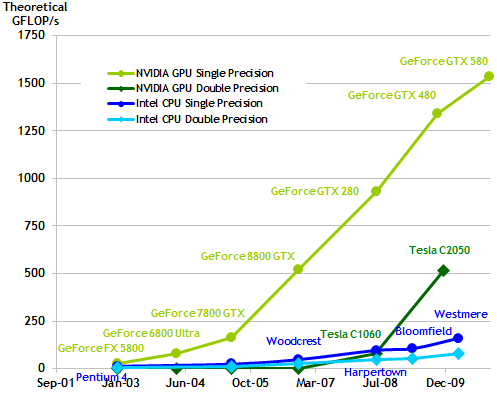
\includegraphics[width=0.48\textwidth]{figures/gpu_vs_cpu.png}
\end{center}
\caption{Performance comparison of GPUs vs CPUs.}
\label{fig:gpu_vs_cpy}
\end{wrapfigure}

Graphical processing units or GPUs are designed to trace rays of light and generate an image. Ray tracing and particle tracking are very similar and because of this, GPUs have the potential to make great particle tracking processors. However, there are some issues with moving to a new architecture. The sheer amount of processing power reduces the time of many computations to the point where moving the data to and from the processor is more expensive than the computation.  The lack of a large cache means that data access patterns and organization are significantly more important. Coupling GPUs and MPI introduces multiple levels of parallelism that have very different characteristics.

The key to developing a high performance particle tracking code is properly decomposing and organizing the problem at each level of the multi-parallel tree. The complexity of the particle mover, collision operator, and timescale of the problem play large roles in how the problem is decomposed. This project will focus on development and performance characterization of generalized mulit-GPU PIC implementation techniques.

\section{Background}
Utilizing GPUs for PIC codes is a relatively recent development which coincides with the accessibility of general purpose gpu (GPGPU) computing. GPGPU computing has evolved rapidly since NVIDIA released the Compute Unified Architecture (CUDA) in 2008. Parallelization of the particle advancing step has been relatively straightforward, however, the developing an efficient charge assign on the GPU is more difficult, unless the particles are sorted. 

There are four main approaches to maintaining a sorted particle list, the particle linked list by Heiko Burau et al \cite{Burau2010}, particle Quicksort by George Stantchev et al \cite{Stantchev2008}, and particle passing by Xianglong Kong et al \cite{Kong2011}, and the full particle sort using a radix sort. Each of these approaches has advantages and disadvantages, and will be characterized based on performance, ease of implementation, and generality. Additional work in the area of GPU PIC codes can be seen in \cite{Aubert2009,Abreu2011,Decyk2011,Joseph2011}.


\section{Objectives}
The goal of this project is to investigate, develop, and characterize a GPU implementation of the PIC method. The code that will serve as the basis for this project is sceptic3D, a 3D electrostatic PIC code used to model ion collection by a sphere in a flowing plasma, further described in \cite{Hutchinson2002,Hutchinson2003,Hutchinson2005,Hutchinson2006,Patacchini2007,Patacchini2010}. GPU versions of specific sub-components of sceptic3D will be implemented using CUDA C, and compared to the original CPU code. Various GPU-PIC implementation techniques will be explored and evaluated based on their performance, ease of implementation, and applicability to a generalized PIC problem. The thesis will detail the development process and the reasoning behind choosing a specific technique for the final sceptic3Dgpu implementation.



%Utilizing GPUs for PIC codes is a relatively recent development which coincides with the accessibility of general purpose gpu (GPGPU) computing. One of the earliest efforts in developing plasma PIC simulations on the GPU is that of George Stantchev et al. In 2008 Stantchev's group published a paper in the \emph{Journal of Parallel Distributed Computing} outlining the development of a fast density accumulation method for PIC implementations on the GPU. Stantchev's group was one of the first to identify the issue of parallelizing the density update and develop a very efficient solution.\cite{Stantchev2008}

%One method used to model plasma behavior is the Particle-In-Cell, or PIC, method. The PIC method can be used to solve a hybrid kinetic/fluid description of plasma physics by following the trajectories of charged particles in self consistent electromagnetic or electrostatic fields. Since individual particle trajectories can be modeled from first principles, the PIC method can used to model a wide variety of geometries and time scales using well defined physical processes. The downside to this method is that it is susceptible to \emph{discrete particle noise}, which is reduced primarily by tracking a very large number of particles. This means that in order to get decent statistics on large, million plus, element meshes, hundreds of millions of particles must be tracked. Tracking millions of particles on a single processor simply is not feasible, fortunately for time scales much less than the inverse plasma frequency, particle trajectories can be taken as completely independent of one another. If the particle trajectories are independent of one another then they can be safely advanced in parallel. The parallel time complexity of advancing the particles is simply $\textcal{O}(n/N_P}$ where $n$ is the number of particles and $N_P$ is the number of processors.

%There is an architecture for which $n \approx N_P$


\section{Schedule}

\begin{description}
\item[September 2011:]\item \indent \vspace{-1cm} \begin{itemize}
		\item	Profile sceptic3D and develop Fortran-CUDA api. 
		\item Compare particle structures, Structure of Arrays vs Array of structures. 
		\item Redesign re-injection technique to be compatible with GPU version. 
	\end{itemize}

\item[October 2011:]\item \indent \vspace{-1cm} \begin{itemize}
		\item Research and test particle sorting methods.  
		\item Implement, debug, and test GPU versions of ptomesh and charge assign subroutines.
	\end{itemize}

\item[November 2011:] Develop and implement GPU particle advancing subroutine.

\item[December 2011:]\item \indent \vspace{-1cm} \begin{itemize}
		\item Enable multi-gpu capabilities. 
		\item Begin GPU implementation of field solve subroutine.
	\end{itemize}

\item[January 2012:]\item \indent \vspace{-1cm} \begin{itemize}
		\item Finish GPU field solve, clean up Makefile.
		\item Perform basic optimizations. 
		\item Begin benchmarking code. Outline thesis. 
		\item Begin Introduction and Implementation chapters. 
	\end{itemize}

\item[February 2012:]\item \indent \vspace{-1cm} \begin{itemize}
		\item Finish performance benchmarks, prepare performance figures.
		\item Start performance chapter.
	\end{itemize}

\item[March 2012:] Complete drafts of Design and Implementation chapters. 

\item[April 2011:] Complete rough draft of thesis.

\item[May 2012:] Revise and submit final draft of thesis. 

\end{description}



\singlespacing
\bibliography{prospectus}
\bibliographystyle{plain}



\end{document}
